
\chapter{Nanostrutture}
Il senso di creare una nanostruttura è quello di cambiare le proprietà del materiale confinandolo dimensionalmente e cambiando quindi la sua densità di stati all'energia di Fermi che è ciò che dona le proprietà ad un materiale. 
\begin{figure} [H]
    \centering
    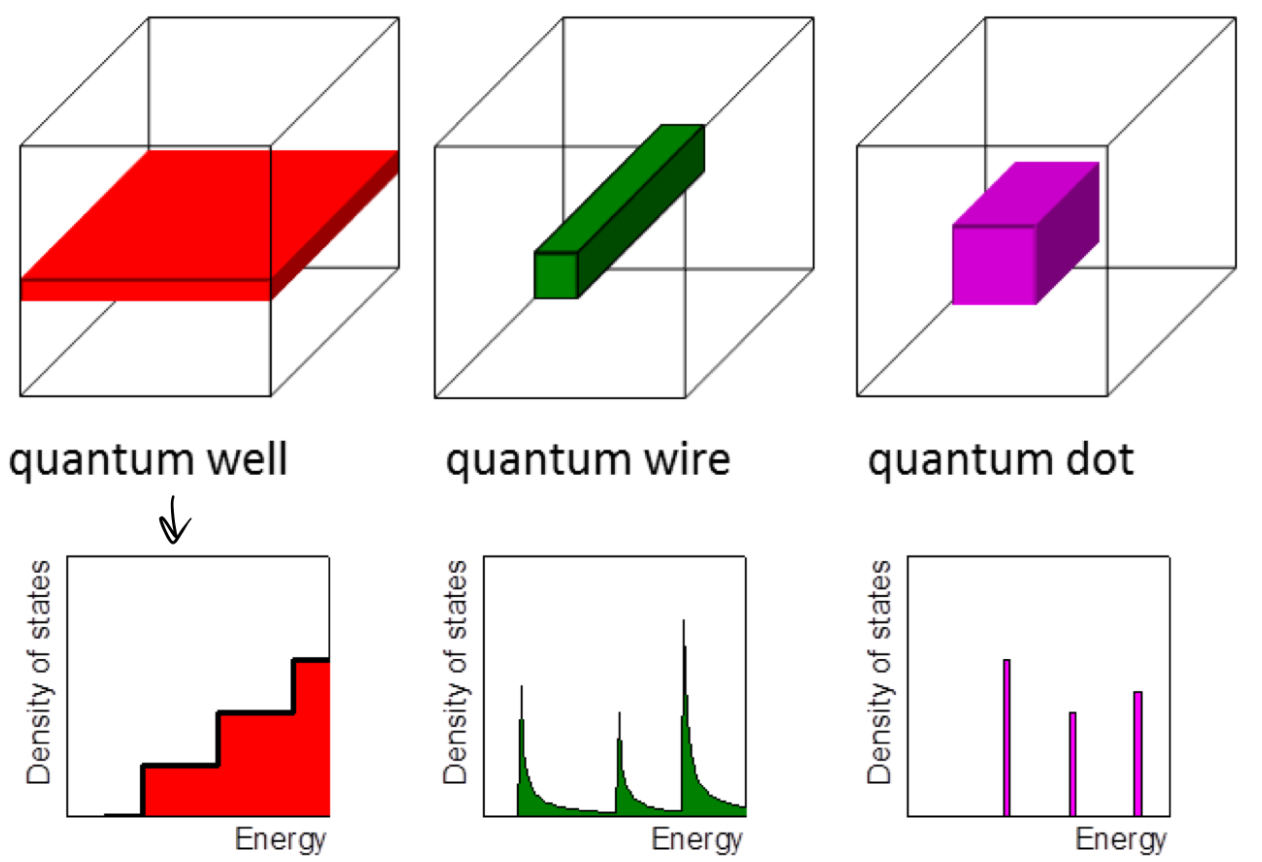
\includegraphics[width=0.5\linewidth]{images/9-Nanostrutture/Nanostr.jpeg}
    \caption{}
    \label{fig:nanostruttura}
\end{figure}

\section{Eterostrutture a confinamento quantico}
Si possono creare delle strutture che combinano un materiale ad alto gap con uno a basso gap, crescendoli su di un substrato layer per layer, creando la struttura in Figura \ref{fig:eterostruttura}
\begin{figure} [H]
    \centering
    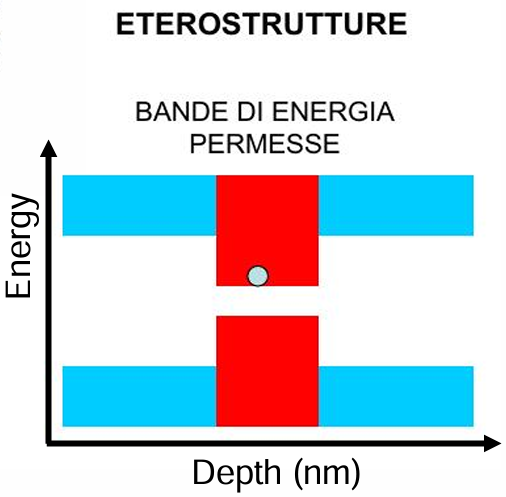
\includegraphics[width=0.4\linewidth]{images/9-Nanostrutture/eterostruttura.png}
    \caption{il materiale azzurro è quello ad alto gap mentre quello rosso è quello a basso gap}
    \label{fig:eterostruttura}
\end{figure} 

L'elettrone non si muove nella zona bianca dell'eterostruttura perché non ho stati permessi
\subsection{Molecular beam epitaxy (MBE)}

La tecnica della \textit{Molecular Beam Epitaxy} (MBE) sfrutta un controllo atomico per la crescita epitassiale di film sottili. Questo documento analizza in maniera dettagliata il processo MBE, focalizzandosi sulla scelta del substrato, l'evaporazione del materiale, il controllo del flusso molecolare e l'importanza delle condizioni in \textit{ultra-alto vuoto} (UHV).

\subsection{Selezione del Substrato}

Il substrato ideale su cui far crescere il film deve essere costituito dallo stesso materiale del film da depositare oppure da un materiale con una costante reticolare simile. Tale compatibilità strutturale è essenziale per:
\begin{itemize}
    \item Minimizzare lo stress reticolare.
    \item Ridurre la formazione di dislocazioni e difetti durante la deposizione.
    \item Favorire una crescita cristallina omogenea e di alta qualità.
\end{itemize}

\subsection{Evaporazione del Materiale}

Il materiale da depositare viene riscaldato all'interno di celle di evaporazione tramite un filamento in tungsteno. L'innalzamento della temperatura induce l'evaporazione del materiale, trasformandolo in un fascio di molecole o atomi.

L'uso del tungsteno, grazie al suo elevato punto di fusione, permette di ottenere:
\begin{itemize}
    \item Una distribuzione stabile ed omogenea dell'energia termica.
    \item Un'evaporazione controllata del materiale.
\end{itemize}

\subsection{Utilizzo dello Shutter}

Prima che il materiale evaporato venga diretto verso il substrato, un \textit{shutter} (otturatore) viene utilizzato per intercettare e controllare il fascio molecolare. In particolare:
\begin{itemize}
    \item Lo shutter permette di bloccare il flusso di molecole fino al momento opportuno.
    \item Una volta aperto, lo shutter consente il passaggio del fascio verso il substrato, garantendo un controllo preciso del tasso di deposizione.
\end{itemize}

\subsection{Ambiente di Ultra-Alto Vuoto (UHV)}

La camera di deposizione è mantenuta in condizioni di ultra-alto vuoto, tipicamente dell'ordine di \(10^{-11}\) mbar, un valore significativamente inferiore rispetto alla pressione atmosferica (circa 1000 mbar). Queste condizioni sono fondamentali per:

\begin{itemize}
    \item \textbf{Prevenzione della contaminazione:} Il vuoto riduce al minimo la presenza di molecole residue che potrebbero contaminare il film sottile.
    \item \textbf{Controllo delle interazioni:} Garantisce che le interazioni tra il fascio molecolare e il substrato avvengano in maniera controllata, evitando reazioni indesiderate.
\end{itemize}

\subsection{Conclusioni}

La MBE rappresenta una tecnica estremamente precisa per la fabbricazione di materiali semiconduttori e sistemi complessi. La combinazione di una selezione accurata del substrato, il controllo termico dell'evaporazione, e l'impiego di uno shutter per regolare il flusso molecolare, consente di ottenere film sottili di alta qualità. Le condizioni in ultra-alto vuoto sono, infine, indispensabili per evitare contaminazioni e assicurare una crescita epitassiale con le proprietà fisiche e strutturali desiderate.
\begin{figure} [H]
    \centering
    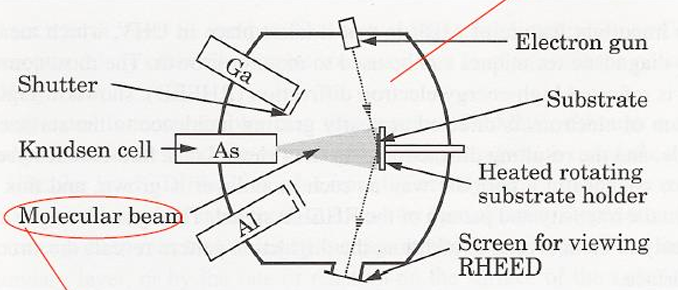
\includegraphics[width=0.8\linewidth]{images/9-Nanostrutture/MBE.png}
    \caption{}
    \label{fig:MBE}
\end{figure} 

\begin{figure} [H]
    \centering
    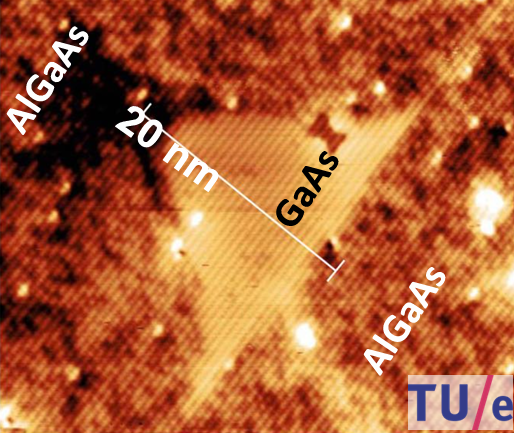
\includegraphics[width=0.5\linewidth]{images/9-Nanostrutture/cross-section.png}
    \caption{l'\ce{AlGaAs} è l'elemento ad alto gap mentre il \ce{GaAs} è quello a basso gap}
    \label{fig:crosss}
\end{figure}

\section{Allineamento delle bande}
Nel progettare eterostrutture a base di semiconduttori, l’obiettivo principale è quello di manipolare i livelli energetici (le bande di conduzione e di valenza) in modo da controllare il comportamento di elettroni e lacune. Ciò si realizza integrando materiali differenti in modo tale che le loro proprietà elettroniche, come il gap di banda e l’affinità elettronica, producano una struttura di bande ingegnerizzata.

\subsection{Regola di Anderson}

Uno degli approcci più utilizzati per stimare l’allineamento delle bande tra due semiconduttori è la \textbf{regola di Anderson}. Secondo questa regola, assumendo che i livelli di energia nel vuoto siano allineati, la differenza tra i livelli della banda di conduzione dei due materiali corrisponde alla differenza nelle loro affinità elettroniche:
\[
\Delta E_c = \chi_1 - \chi_2
\]
dove $\chi$ è l'affinità elettronica. Questa regola fornisce una stima iniziale utile per progettare eterogiunzioni, anche se non tiene conto di effetti interfaccia come stati interfaccia o polarizzazione spontanea.

La scelta della coppia di materiali non deve quindi basarsi solo sulla compatibilità del passo reticolare, ma anche sull’allineamento energetico, in modo da garantire un efficiente trasporto di carica.

\subsection{Effetti del disallineamento reticolare}

È comunque possibile far crescere materiali con un passo reticolare diverso, ma questo genera disallineamenti nella struttura cristallina, con la formazione di difetti strutturali. Tali difetti possono comportare la presenza di zone che intrappolano cariche, note come \textbf{zone morte}.
\\
In alcuni casi, queste zone morte possono risultare utili: introducono livelli energetici intermedi che permettono l’assorbimento di fotoni con energie diverse. \\
Questo principio viene sfruttato per aumentare l’efficienza delle celle fotovoltaiche, consentendo l’assorbimento di una porzione più ampia dello spettro solare.

\subsection{Quantum well}

Una particolare eterostruttura di interesse è la \textbf{quantum well}, ovvero una struttura in cui un materiale a gap minore è confinato tra due materiali a gap maggiore. Questo porta al confinamento quantistico degli elettroni lungo una direzione (solitamente la direzione di crescita epitassiale), lasciando libertà di movimento nelle altre due dimensioni.

Il confinamento quantistico porta alla quantizzazione dei livelli energetici nella banda di conduzione e di valenza. Modificando lo spessore del pozzo quantico, è possibile controllare direttamente l’energia di questi livelli.

\subsection{Esperimenti di fotoluminescenza}

In esperimenti di fotoluminescenza, si irraggia la quantum well con luce avente energia $h\nu > E_{gap}$ del materiale, promuovendo elettroni nella banda di conduzione. Alcuni di questi elettroni vengono confinati negli stati quantizzati del pozzo.

Successivamente, gli elettroni decadono verso la banda di valenza, emettendo fotoni con energia corrispondente alla differenza tra i livelli quantizzati. Controllando la larghezza del pozzo, si controlla anche l’energia dei fotoni emessi, senza dover modificare la composizione chimica del materiale.

\subsection{Conclusioni}

L’ingegnerizzazione delle eterostrutture richiede un’attenta valutazione sia del passo reticolare che dell’allineamento delle bande. Difetti strutturali possono essere sfruttati per aumentare l’assorbimento spettrale, mentre le quantum well offrono un controllo preciso delle proprietà ottiche attraverso la sola variazione geometrica. Questi concetti sono fondamentali per lo sviluppo di dispositivi optoelettronici avanzati come laser a semiconduttore, LED e celle solari multi-giunzione.


\section{Determinare lo stato elettronico}
Supponiamo di trattare la nanostruttura come una perturbazione, per cui avremo:
\begin{equation}
    \begin{split}
        &(H_{id} + V_{per}) \cdot \xi(\vec{r}) = E \cdot \xi(\vec{r})\\
        &H_{id} \cdot \psi_{n,k}= \varepsilon\cdot \psi_{n,k} \hspace{0.4cm}\psi_{n,k}= e^{i\vec{k}\cdot\vec{r}}\cdot u_{n,k}\hspace{0.3cm} \textbf{stati di Bloch} \\
    \end{split}
\end{equation}
Applichiamo la teoria perturbativa per semplicità nel caso 1-D:
\begin{equation}
    \xi(x) = \sum_k \int_{-\frac{\pi}{a}}^{\frac{\pi}{a}} \chi_n(k)\cdot \psi_{n,k}(x)\cdot \frac{\d{k}}{2\pi}y
\end{equation}
\textbf{Prima approssimazione}: banda singola, ossia trascuro i termini al di fuori della banda di conduzione.\\
\textbf{Seconda approssimazione}: consideriamo la perturbazione grande rispetto al passo reticolare $L>>a \implies k$ sta attorno al minimo della banda ossia $k<<\frac{2\pi}{a}$, $k\approx 0$. Ciò implica che le autofunzioni $u_{c,k}$ variano debolmente con $k$, ossia possiamo scrivere:\\
\[\psi_{c,k} = u_{c,k}\cdot e^{ikx} \approx \psi_{c,0} \cdot e^{ikx} \implies \xi(x) \approx \psi_{c,0}(x) \cdot \int_{-\frac{\pi}{a}}^{\frac{\pi}{a}}\chi_c(k) \cdot e^{ikx}\cdot \frac{\d{k}}{2\pi} = \psi_{c,0}\cdot \chi_c(x)\]
        
Dove $\chi_c(x)$ è la trasformata di fourier e prende nome di \textbf{funzione inviluppo} , applichiamo ora la prima parte della Hamiltoniana:
\[H_{id.} \cdot \xi(x) = \int_{-\frac{\pi}{a}}^{\frac{\pi}{a}}\chi_c(k) \cdot H_{id.} \cdot \psi_{c,k}(x)\cdot \frac{\d{k}}{2\pi}  = \int_{-\frac{\pi}{a}}^{\frac{\pi}{a}}\chi_c(k) \cdot \varepsilon_{c,k}\cdot u_{c,k}\cdot e^{ikx}\cdot \frac{\d{k}}{2\pi} \]
\[\approx \psi_{c,0} \int \chi_c(k) \cdot \varepsilon_{c,k} \cdot e^{ikx}\cdot \frac{\d{k}}{2\pi}  \]
Dove gli estremi vanno via in quanto $k\approx 0$
\[\varepsilon_c(k) = \sum_ma_m^c\cdot k^m \approx E_c + \frac{\hbar^2}{2m^*}\cdot k^2 \hspace{0.3cm} \text{con} \hspace{0.3cm} m^* \approx \frac{d^2\varepsilon}{d^2x} \]
\[\implies  E_c \cdot \psi_{c,0} \int \chi_c(k) \cdot e^{ikx}\cdot \frac{\d{k}}{2\pi} + \psi_{c,0} \frac{\hbar^2}{2m^*}\int \chi_c(k) \cdot k^2 \cdot e^{ikx}\cdot \frac{\d{k}}{2\pi}  \]
\[=E_c \cdot \psi_{c,0} \int \chi_c(k) \cdot e^{ikx}\cdot \frac{\d{k}}{2\pi} + \psi_{c,0} \frac{\hbar^2}{2m^*} \cdot \biggr(-\frac{d^2}{d^2x}\cdot \chi_c(x)\biggr)\]
 
Per cui l'equazione agli autovalori $(H_{id}+V_{per.})\cdot \xi = E \cdot \xi$ diventa:\\
\begin{equation}
    \begin{split}
        &\psi_{c,0}(x)\cdot \biggr(E_c-\frac{\hbar^2}{2m^*}\cdot \frac{d^2}{d^2x}\biggr)\cdot \chi_c(x) + V_{per.}\cdot \psi_{c,0}(x) \cdot \chi_c(x) = E \cdot \psi_{c,0}(x) \cdot \chi_c(x)\\
        &\biggr(-\frac{\hbar^2}{2m^*}\cdot \frac{d^2}{d^2x}+V_{per.}\biggr)\cdot \chi_c(x) = (E-E_c)\cdot \chi_c(x)\\
    \end{split}
\end{equation}
\\\\
\textbf{Quindi si ottiene un'equazione di shrodinger sottoposta ad un potenziale perturbativo esterno con autostato la funzione inviluppo $\chi_c(x)$}, osserviamo che non coincide con l'autofunzione del sistema $\xi(x)$, per cui non che deve essere necessariamente una funzione continua con derivata continua.\\\\

\subsection{Esempio: Quantum well a pareti infinite $D=2$}
Supponiamo di avere quindi una buca di potenziale con pareti idealmente infinite $V_0 \to \infty$ tra $-\frac{a}{2}<z<\frac{a}{2}$, le soluzioni avranno la forma:
\begin{equation}
    \begin{split}
        & \phi_n(z) \begin{cases}
            \sqrt{\frac{2}{a}}\cdot \cos\biggr(\frac{n\pi z}{a}\biggr) \hspace{0.3cm} \text{n dispari}\\
            \sqrt{\frac{2}{a}}\cdot \sin\biggr(\frac{n\pi z}{a}\biggr) \hspace{0.3cm} \text{n pari}
        \end{cases}\\
        &\varepsilon_n = \frac{\hbar^2}{2m_e}\cdot \biggr(\frac{n\pi}{a}\biggr)^2\\
    \end{split}
\end{equation}

\subsection{Esempio: Quantum well a pareti finite $(D=2)$}
Per descrivere una Quantum well a pareti finite supponiamo di considerare un sistema in cui l'energia in funzione della coordinata $z$ sia suddivisa in 3 zone: una prima zona che corrisponde ad una energia $V_0$ (barriera), una zona intermedia a energia nulla compresa tra $-\frac{a}{2}< z <\frac{a}{2}$ (fondo della banda di conduzione della quantum well) e una terza zona a energia $V_0$ (barriera).\\
Consideriamo le seguenti ipotesi:\\
\begin{enumerate}
    \item tutte le energia sono misurate dal fondo della quantum well.
    \item la funzione $\psi_{c,0}$ è la stessa per tutte le tre zone con $\xi = \psi_{c,0}\cdot \chi_c(x) $ autostato del sistema.
    \item la massa efficacie $m^*_e$ è la stessa per tutte le tre zone
    \item gli stati a energia $\varepsilon< V_0$ sono \textbf{stati legati} mentre quelli con $\varepsilon> V_0$ sono \textbf{stati delocalizzati}.
\end{enumerate}
\begin{equation}
    \begin{split}
        &\psi_2(z) = C \cdot \begin{cases}
            \cos(kz) \\
            \sin(kz) \end{cases}\hspace{0.3cm}\text{dentro alla quantum well}\\
        &-\frac{\hbar^2}{2m_e}\cdot \frac{d^2}{d^2z}\psi_{1,3}(z)+V_0\cdot\psi_{1,3}(z) = \varepsilon \cdot \psi_{1,3}(z) \hspace{0.3cm}\text{fuori dalla quantum well}\\
        &\psi_1 = D\cdot e^{Kz} \hspace{0.9cm} \psi_3 =D\cdot  e^{-Kz}\hspace{0.9cm}\frac{\hbar^2K^2}{2m_e}= V_0-\varepsilon =B\\
    \end{split}
\end{equation}
Studiamo il caso per $z>\frac{a}{2}$ e per simmetria possiamo dedurre il caso di $z<-\frac{a}{2}$, imponiamo quindi la continuità della funzione e della derivata nel punto di contatto $z=\frac{a}{2}$.\\
\begin{equation}
    \begin{split}
        &\psi\biggr(\frac{a}{2}\biggr)=C\cdot \begin{cases}
            \cos(\frac{ka}{2})\\
            \sin(\frac{ka}{2})\end{cases} = D \cdot e^{-\frac{Ka}{2}}\\
        &\frac{d\psi}{dz}\biggr|_{z=\frac{a}{2}} = C\cdot k \cdot \begin{cases} -\sin(\frac{ka}{2}) \\
        \cos(\frac{ka}{2})  \end{cases} = -D\cdot K\cdot e^{-\frac{Ka}{2}}\\
        &k\cdot \begin{cases}-\tan(\frac{ka}{2})\\ \cot(\frac{ka}{2}) \end{cases}=-K\hspace{0.3cm}\text{dividendo membro a membro le due eq.}\\
        &\begin{cases}\tan(\frac{ka}{2})\\ -\cot(\frac{ka}{2}) \end{cases}= \frac{K}{k} = \frac{1}{k}\cdot \sqrt{\frac{2m_e}{\hbar^2}\cdot (V_0-\varepsilon)}= \sqrt{\frac{2m_eV_0}{\hbar^2k^2}-1}\\    
        &\begin{cases}\tan(\theta)\\ -\cot(\theta) \end{cases}= \sqrt{\frac{2m_eV_0\cdot a^2}{2\hbar^2}\cdot \frac{1}{\theta^2}-1}= \sqrt{\frac{\theta_0^2}{\theta^2}-1}\hspace{0.3cm}\text{definendo}\hspace{0.3cm}\theta= \frac{ka}{2} \hspace{0.3cm}\theta_0^2= \frac{m_eV_0a^2}{2\hbar^2}\\       
    \end{split}
\end{equation}
\\
\begin{figure} [H]
    \centering
    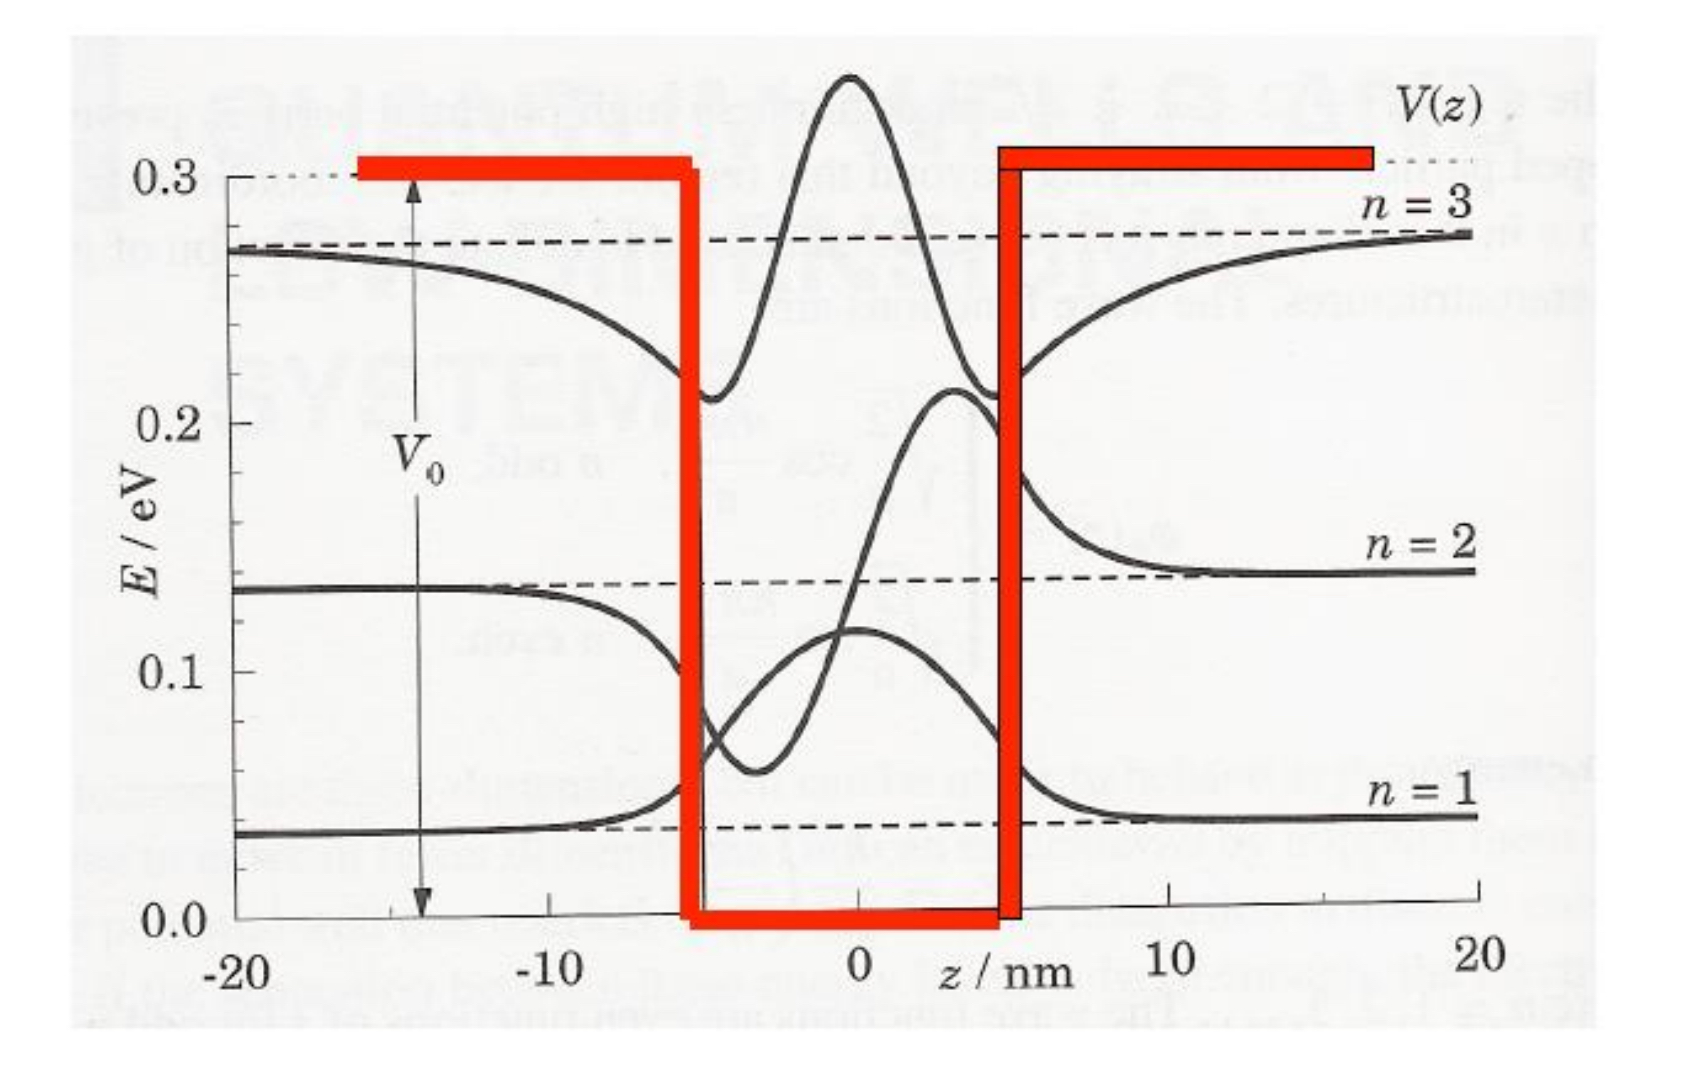
\includegraphics[width=0.7\linewidth]{images/9-Nanostrutture/IMG_1788.jpg}
    \caption{funzioni d'onda risultanti}
\end{figure}
\begin{figure} [H]
    \centering
    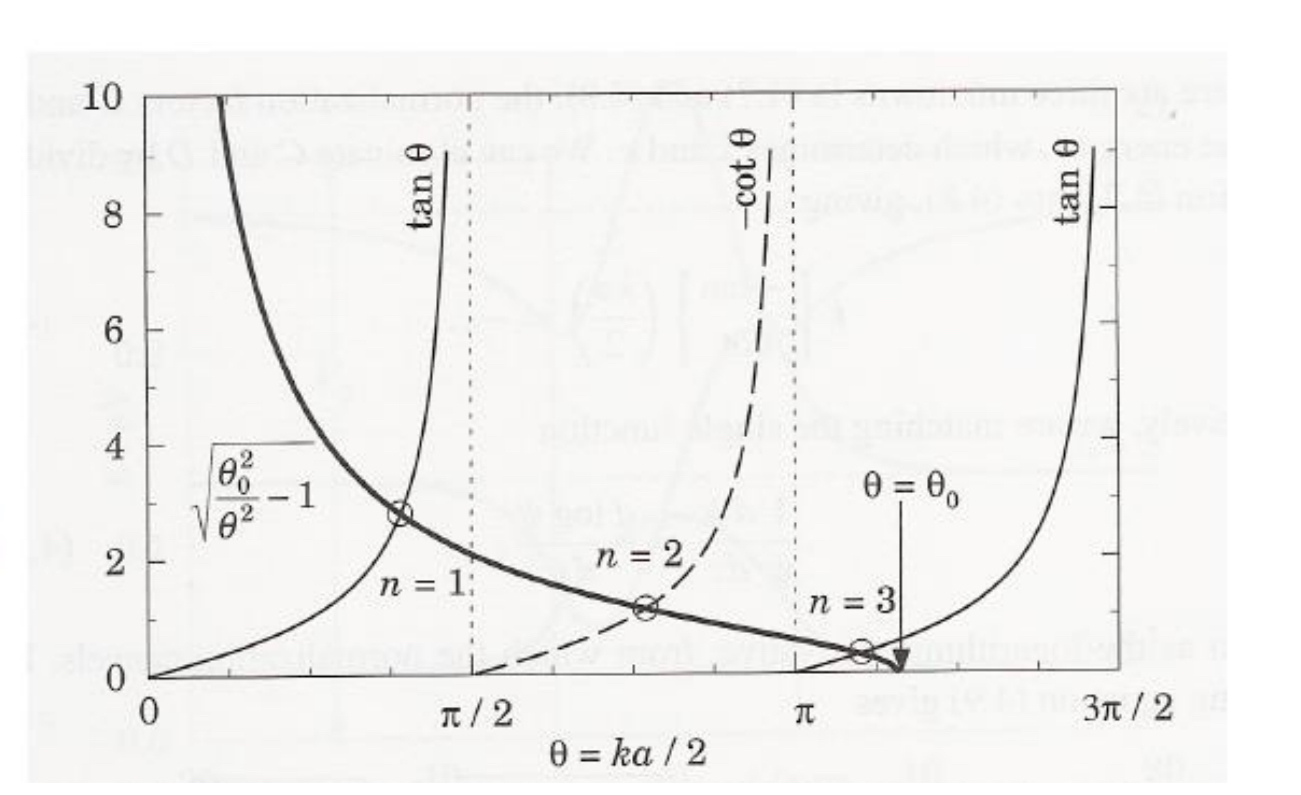
\includegraphics[width=0.7\linewidth]{images/9-Nanostrutture/IMG_1790.jpg}
    \caption{Risoluzione grafica per ricavare $\theta$}
\end{figure}

Considerazioni:
\begin{enumerate}
    \item Il numero di soluzioni dell'equazioni è dato da $\frac{2}{\pi}\cdot \theta_0 = \frac{2}{\pi}\cdot \frac{m_eV_0a^2}{2\hbar^2}$ quindi esiste sempre almeno una soluzione (\textbf{una QW ha sempre uno stato legato}).
    \item Per una QW poco profonda (un solo stato legato) si dimostra che l'energia di legame B dello stato legato è: $B= V_0-\varepsilon \approx \frac{m_eV_0^2a^2}{2\hbar^2}$.
    \item Per un certo stato legato, la probabilità di trovare l'elettrone dentro la QW è: $\int_{-\frac{a}{2}}^\frac{a}{2}|\psi(z)|^2\cdot dz \cdot \bigl[\int_{-\frac{a}{2}}^{\frac{a}{2}}|\psi(z)|^2\cdot dz\bigr]^{-1}$ quindi aumentare la profondità della QW, equivale ad aumentare $\varepsilon$, $B$ e $k$, ossia lo stato è meglio confinato. 
    \item Gli stati a piccolo valore di $n$ sono meno penetranti negli slab di barriera.
\end{enumerate}

\textbf{Il problema completo corrisponde a considerare un'equazione agli autovalori in tre dimensioni in cui la variazione del potenziale avviene solo lungo una direzione $V(x,y,z) =V(z)$}, siccome l'elettrone è libero nel piano $(x,y)$, la soluzione generale avrà la forma: 
\[\psi(x,y,z) = e^{ik_x\cdot x} \cdot e^{ik_y\cdot y}\cdot u(z)\]
sostituendo si ottiene:
\begin{equation}
    \bigl[-\frac{\hbar^2}{2m}\cdot \frac{d^2}{d^2z}+V(z)\bigr]\cdot u(z) = \varepsilon\cdot u(z) \hspace{0.4cm} \varepsilon = E - \frac{\hbar^2k_x^2}{2m}-  \frac{\hbar^2k_y^2}{2m}
\end{equation}
Questa equazione corrisponde a quella che abbiamo risolto sopra per la QW a pareti infinite o finite e conosciamo le soluzioni $u_n(z)$ corrispondenti a stati legati, il sistema è quindi caratterizzato da 3 numeri quantici $k_x,k_y,n$:
\begin{equation}
    \psi_{k_x,k_y,n}(x,y,z) = e^{ik_x\cdot x} \cdot e^{ik_y\cdot y}\cdot u_n(z) \hspace{0.5cm} E_n(k_x,k_y)= \varepsilon_n + \frac{\hbar^2k_x^2}{2m_e} + \frac{\hbar^2k_y^2}{2m_e}
\end{equation}
\begin{figure} [H]
    \centering
    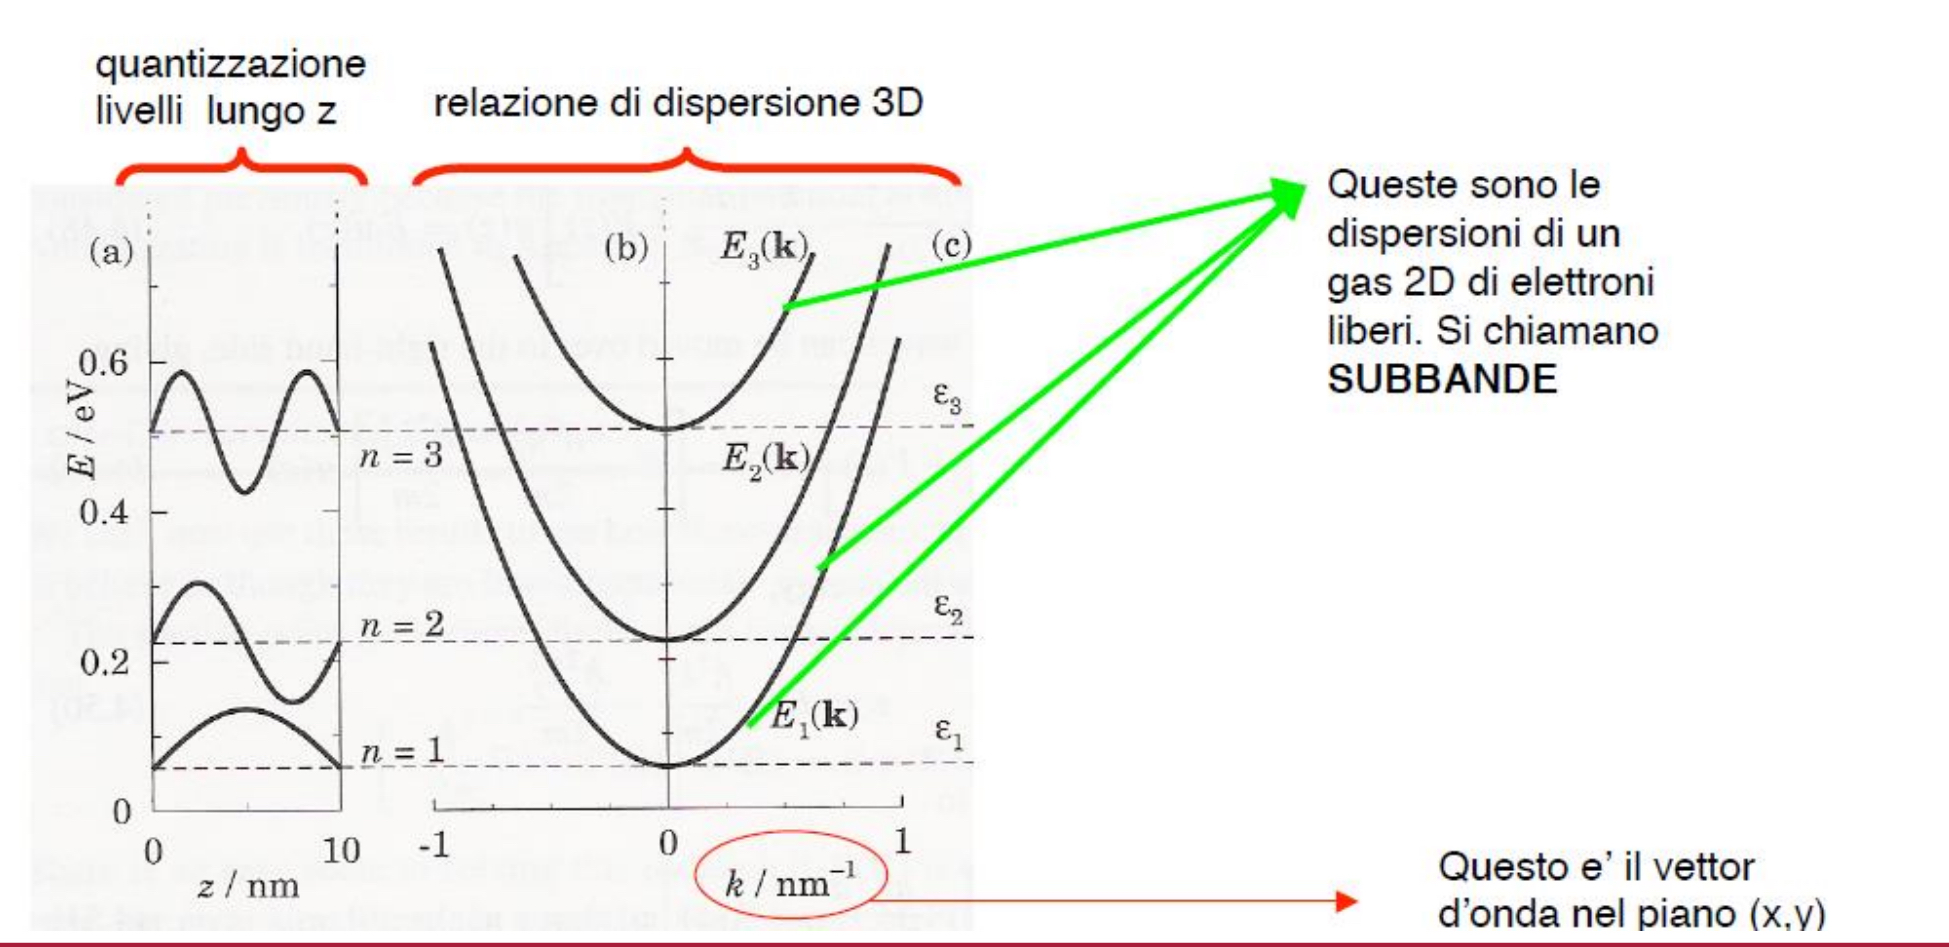
\includegraphics[width=1\linewidth]{images/9-Nanostrutture/IMG_1792.jpg}
\end{figure}
\begin{figure} [H]
    \centering
    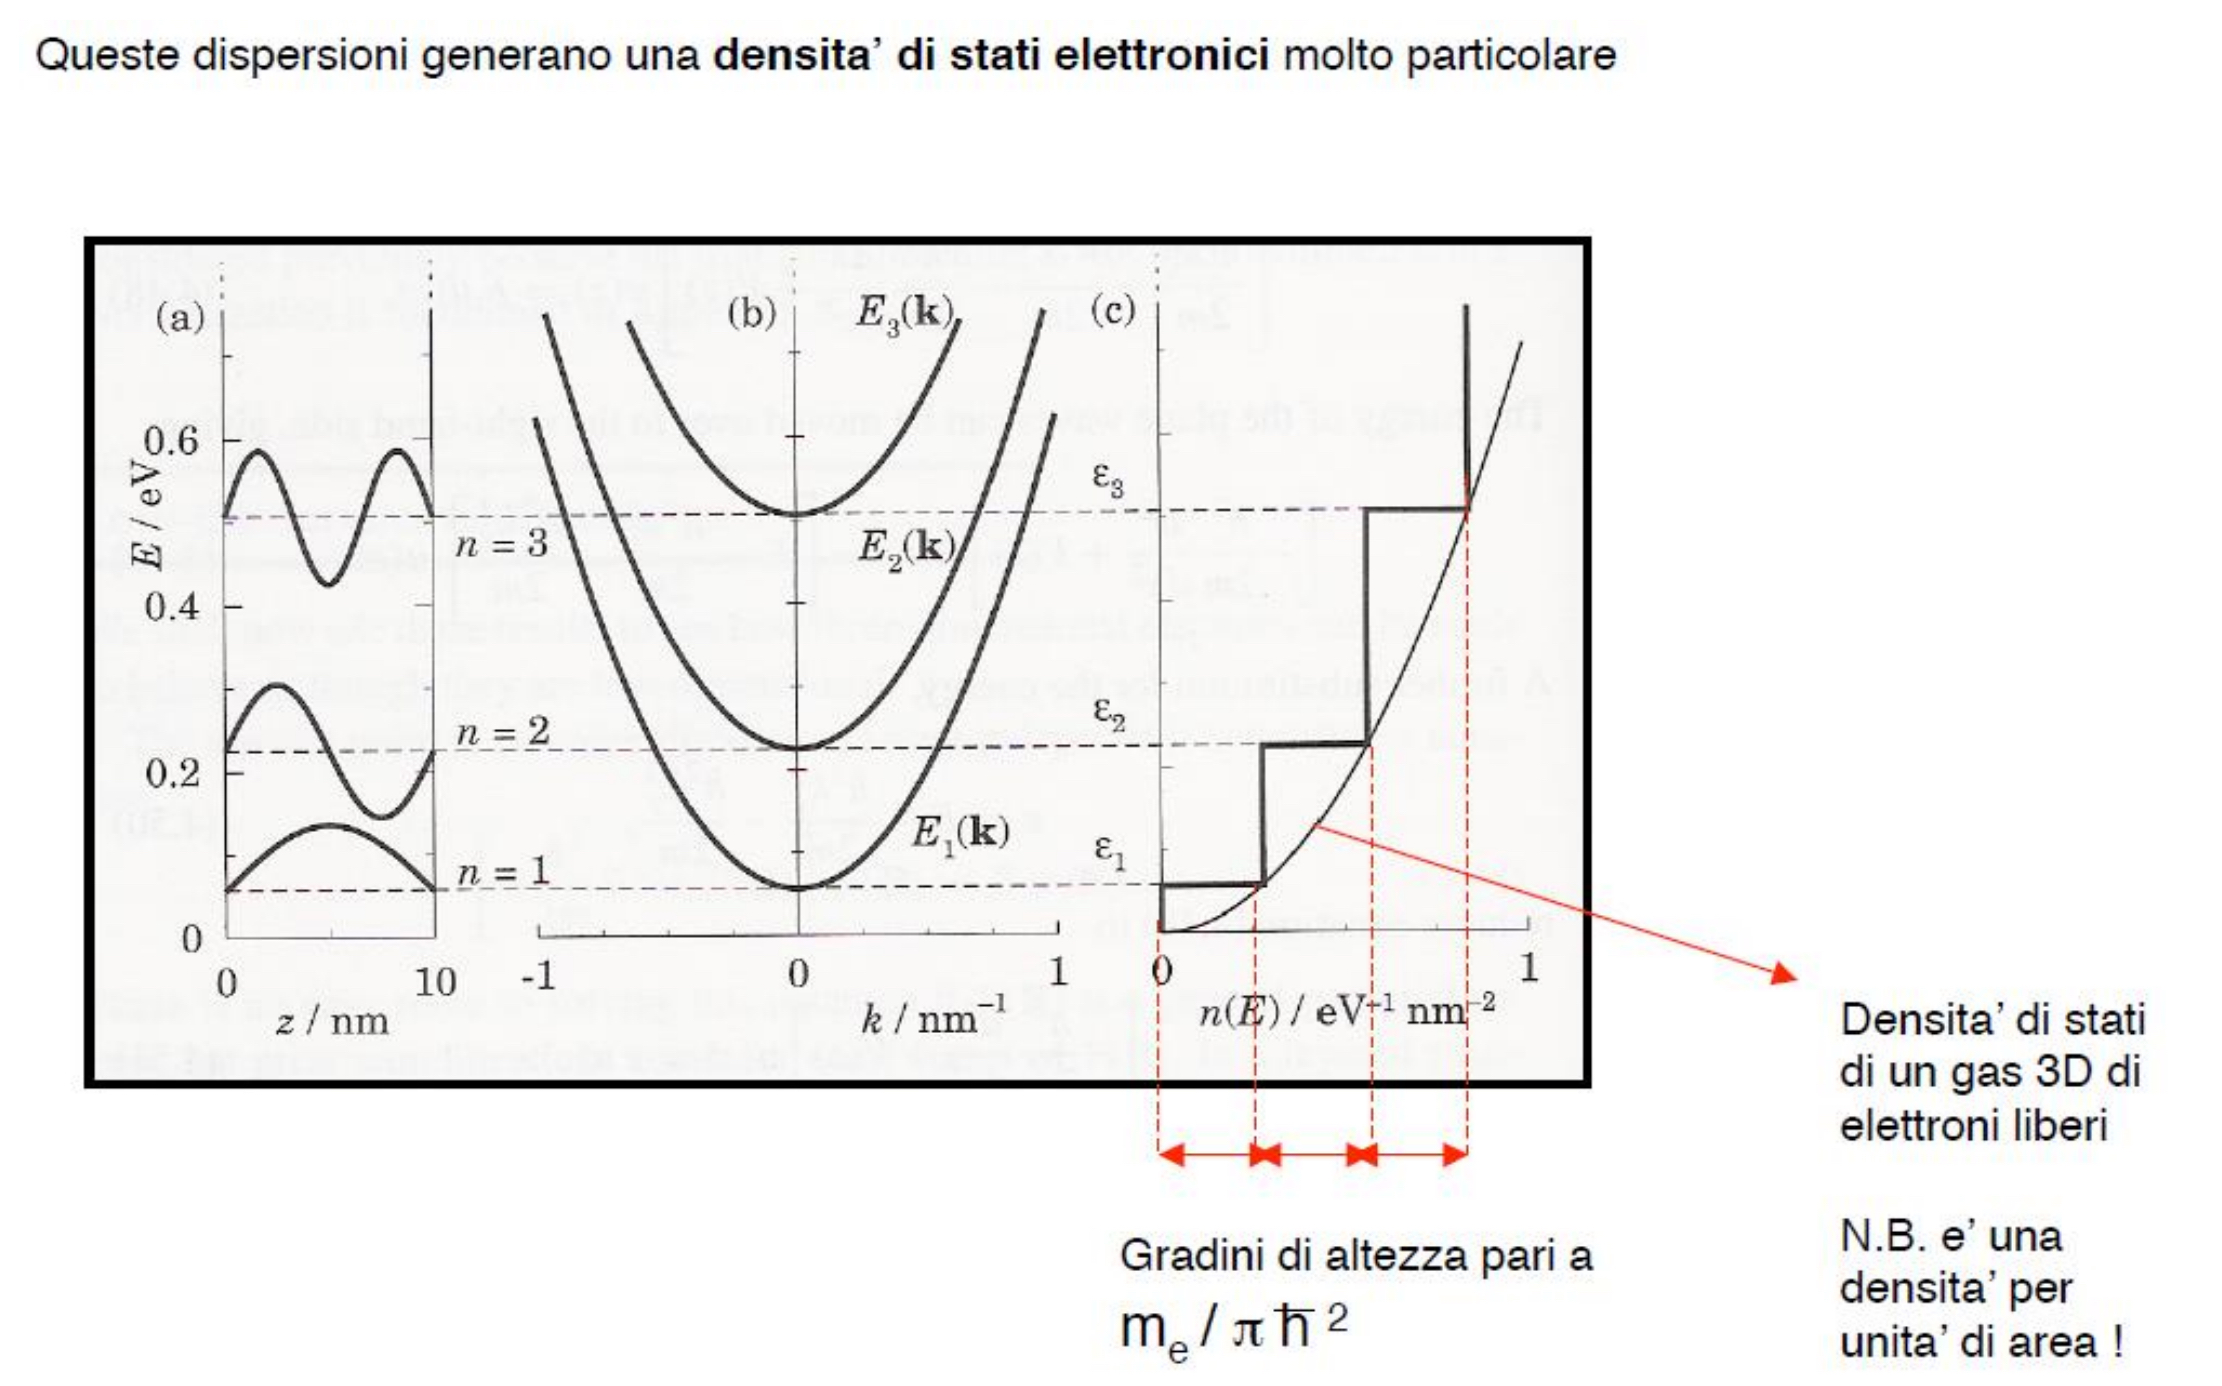
\includegraphics[width=1 \linewidth]{images/9-Nanostrutture/IMG_1793.jpg}
\end{figure}

\section*{Quantum Well a Pareti Finite ($D=2$)}
Si consideri un sistema in cui il potenziale $V(z)$ è suddiviso in tre zone:
\begin{enumerate}
    \item \textbf{Zona 1:} $z < -\frac{a}{2}$ con $V(z) = V_0$ (barriera inferiore);
    \item \textbf{Zona 2:} $-\frac{a}{2} < z < \frac{a}{2}$ con $V(z)=0$ (interno della quantum well, fondo della banda di conduzione);
    \item \textbf{Zona 3:} $z > \frac{a}{2}$ con $V(z) = V_0$ (barriera superiore).
\end{enumerate}
\textbf{Ipotesi:}
\begin{itemize}
    \item Tutte le energie sono misurate rispetto al fondo della quantum well (cioè, $V=0$ nella zona interna).
    \item La massa efficace $m_e^*$ è la stessa in tutte le regioni.
    \item Gli stati con energia $\varepsilon<V_0$ sono \emph{stati legati} (la funzione d'onda decresce esponenzialmente nelle barriere), mentre quelli con $\varepsilon > V_0$ sono \emph{stati delocalizzati}.
\end{itemize}
\subsection*{Soluzione dell'Equazione di Schrödinger}
\subsubsection*{1. Zona Interna della Quantum Well ($-\frac{a}{2} < z < \frac{a}{2}$)}
Nel vano della well il potenziale è nullo e l'equazione stazionaria diventa:
\[
-\frac{\hbar^2}{2m_e}\frac{d^2}{dz^2}\psi_2(z) = \varepsilon\, \psi_2(z).
\]
La soluzione generale è data da:
\[
\psi_2(z)= C\cdot
\begin{cases}
\cos(kz) & \text{(soluzione pari)},\\[1mm]
\sin(kz) & \text{(soluzione dispari)},
\end{cases}
\]
con
\[
k=\sqrt{\frac{2m_e\varepsilon}{\hbar^2}}.
\]

\subsubsection*{2. Zone Esterne (Barriere, $z < -\frac{a}{2}$ e $z > \frac{a}{2}$)}
Per $z$ al di fuori della well il potenziale è costante, $V(z)=V_0$, e l'equazione diventa:
\[
-\frac{\hbar^2}{2m_e}\frac{d^2}{dz^2}\psi_{1,3}(z) + V_0\,\psi_{1,3}(z)= \varepsilon\,\psi_{1,3}(z).
\]
Per stati legati, in cui $\varepsilon<V_0$, si scrive:
\[
-\frac{\hbar^2}{2m_e}\frac{d^2}{dz^2}\psi_{1,3}(z) = (\varepsilon-V_0)\, \psi_{1,3}(z).
\]
Definendo
\[
\frac{\hbar^2K^2}{2m_e} = V_0-\varepsilon \quad \Longrightarrow \quad K=\sqrt{\frac{2m_e(V_0-\varepsilon)}{\hbar^2}},
\]
le soluzioni decrescenti sono:
\[
\psi_1(z)= D\cdot e^{Kz} \quad (z< -\tfrac{a}{2}), \quad \psi_3(z)= D\cdot e^{-Kz}\quad (z>\tfrac{a}{2}).
\]

\subsection*{Condizioni al Contorno}
Per garantire la regolarità della soluzione si impongono la continuità della funzione d'onda e della sua derivata nei punti di confine $z=\pm \frac{a}{2}$. Consideriamo il caso $z=\frac{a}{2}$ (il caso $z=-\frac{a}{2}$ segue per simmetria).

\subsubsection*{Continuità della Funzione}
Si ha:
\[
\psi_2\Bigl(\frac{a}{2}\Bigr)= \psi_3\Bigl(\frac{a}{2}\Bigr),
\]
da cui:
\[
C\cdot
\begin{cases}
\cos\left(\frac{ka}{2}\right) & \text{(soluzione pari)},\\[1mm]
\sin\left(\frac{ka}{2}\right) & \text{(soluzione dispari)}
\end{cases}
= D\cdot e^{-K\frac{a}{2}}.
\]
\subsubsection*{Continuità della Derivata}
Si richiede:
\[
\frac{d\psi}{dz}\Big|_{z=\frac{a}{2}^-} = \frac{d\psi}{dz}\Big|_{z=\frac{a}{2}^+}.
\]
Per la regione interna (zona 2) si ha:
\[
\frac{d\psi_2}{dz}\Big|_{z=\frac{a}{2}} = C\cdot k\cdot
\begin{cases}
-\sin\left(\frac{ka}{2}\right) & \text{(soluzione pari)},\\[1mm]
\cos\left(\frac{ka}{2}\right) & \text{(soluzione dispari)},
\end{cases}
\]
mentre per la zona esterna (zona 3), derivando l'esponenziale, si ottiene:
\[
\frac{d\psi_3}{dz}\Big|_{z=\frac{a}{2}} = -D\cdot K\cdot e^{-K\frac{a}{2}}.
\]

\subsubsection*{Equazioni di Quantizzazione}

Dividendo l'equazione della derivata per quella della funzione (in modo da eliminare le costanti $C$ e $D\cdot e^{-K\frac{a}{2}}$) si ottengono due casi:
\paragraph{Soluzione Pari}
\[
\frac{-C\,k\,\sin\left(\frac{ka}{2}\right)}{C\,\cos\left(\frac{ka}{2}\right)} = -K \quad \Longrightarrow \quad k\, \tan\left(\frac{ka}{2}\right)= K.
\]
\paragraph{Soluzione Dispari}
\[
\frac{C\,k\,\cos\left(\frac{ka}{2}\right)}{C\,\sin\left(\frac{ka}{2}\right)} = -K \quad \Longrightarrow \quad -k\,\cot\left(\frac{ka}{2}\right)= K.
\]
Definendo l'angolo adimensionale
\[
\theta = \frac{ka}{2},
\]
le condizioni diventano:
\[
\begin{cases}
\tan(\theta)=\dfrac{K}{k} & \text{(stato pari)}, \\[2mm]
-\cot(\theta)=\dfrac{K}{k} & \text{(stato dispari)}.
\end{cases}
\]
Notiamo che, essendo
\[
k=\sqrt{\frac{2m_e\varepsilon}{\hbar^2}} \quad \text{e} \quad K=\sqrt{\frac{2m_e(V_0-\varepsilon)}{\hbar^2}},
\]
possiamo scrivere:
\[
\frac{K}{k} = \sqrt{\frac{V_0-\varepsilon}{\varepsilon}}.
\]
Introducendo il parametro adimensionale
\[
\theta_0^2=\frac{m_eV_0a^2}{2\hbar^2},
\]
si ottiene:
\[
\frac{K}{k} = \sqrt{\frac{\theta_0^2}{\theta^2} -1}.
\]
Le equazioni trascendenti risultanti sono:
\[
\begin{cases}
\tan(\theta)=\sqrt{\dfrac{\theta_0^2}{\theta^2}-1} & \text{(stato pari)}, \\[2mm]
-\cot(\theta)=\sqrt{\dfrac{\theta_0^2}{\theta^2}-1} & \text{(stato dispari)}.
\end{cases}
\]
\begin{figure}[h]
\centering
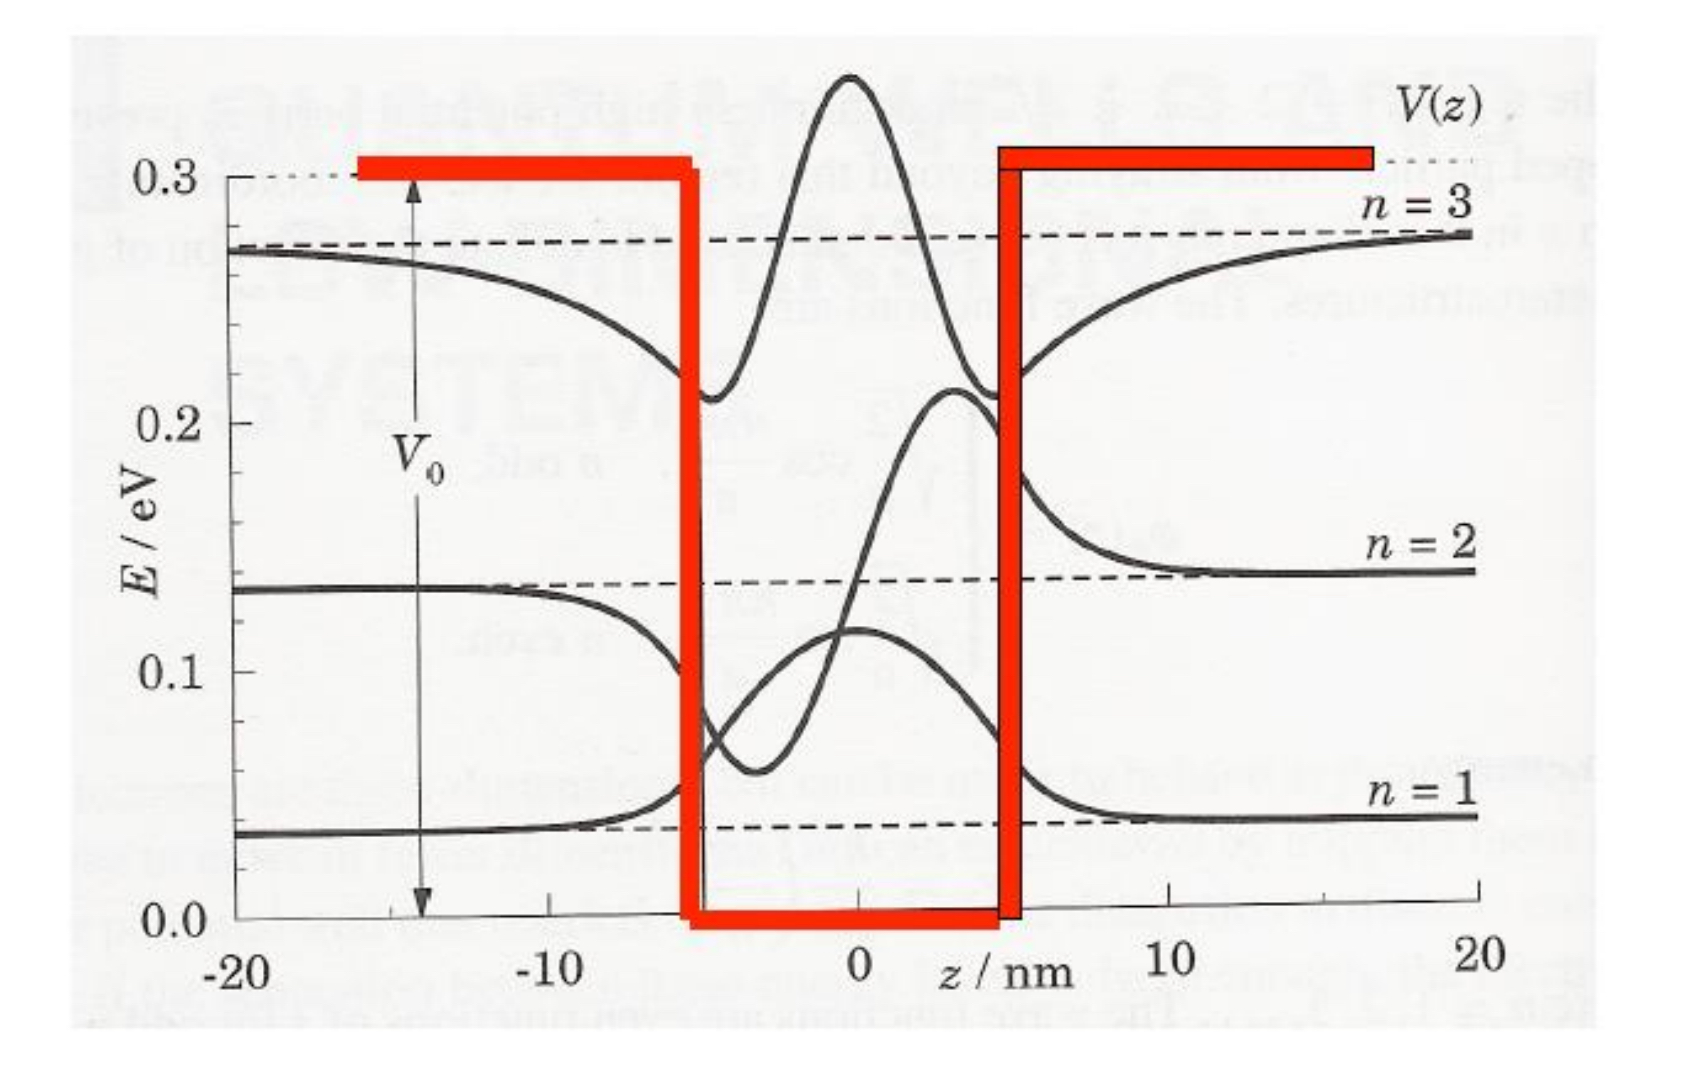
\includegraphics[width=0.7\linewidth]{images/9-Nanostrutture/IMG_1788.jpg}
\caption{Andamento della funzione d'onda all'interno e all'esterno della QW.}
\end{figure}

\begin{figure}[h]
\centering
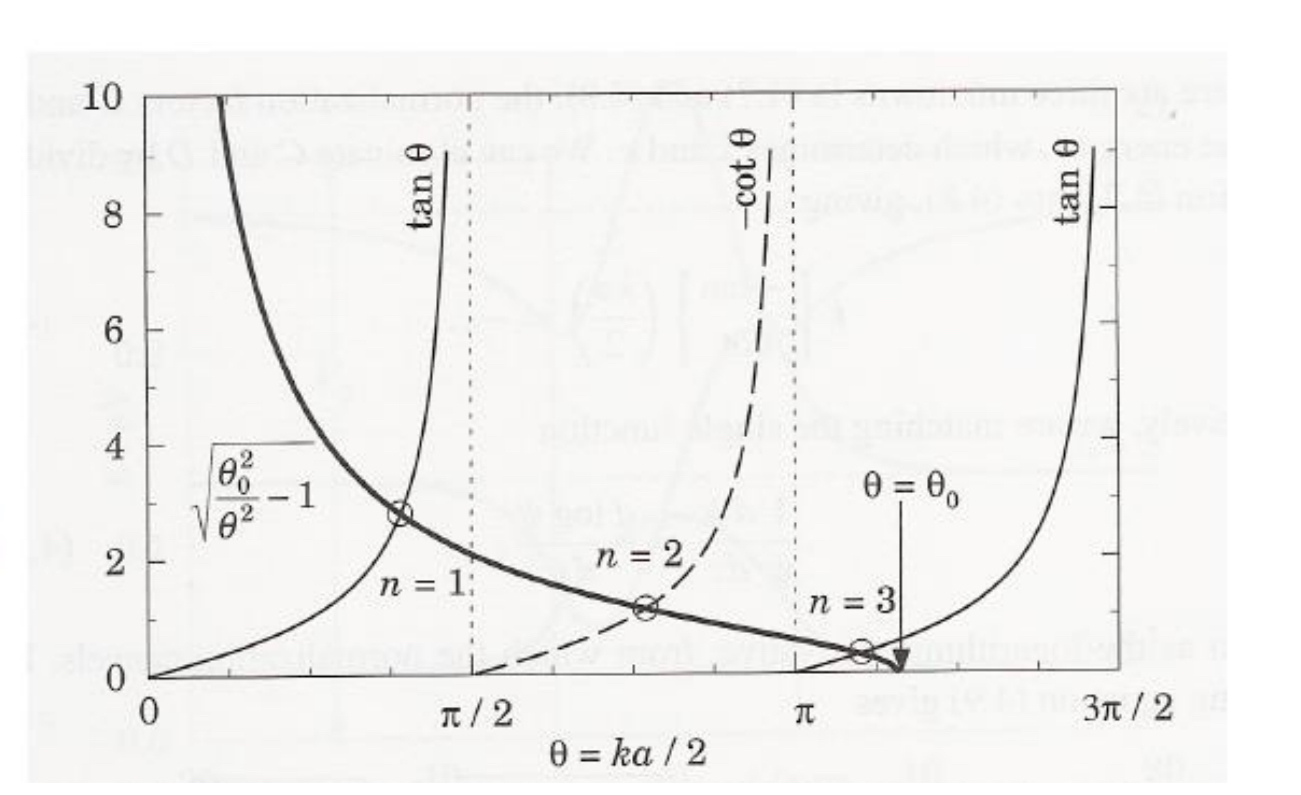
\includegraphics[width=0.7\linewidth]{images/9-Nanostrutture/IMG_1790.jpg}
\caption{Risoluzione grafica per determinare $\theta$.}
\end{figure}

\subsection*{Interpretazione dei Risultati}
\begin{enumerate}
    \item \textbf{Numero di Soluzioni:} \\
    L'equazione trascendente mostra che il numero di soluzioni (stati legati) è approssimativamente:
    \[
    N \approx \frac{2\theta_0}{\pi} = \frac{2}{\pi}\sqrt{\frac{m_eV_0a^2}{2\hbar^2}},
    \]
    garantendo almeno una soluzione, ossia, una quantum well ha sempre almeno uno stato legato.
    
    \item \textbf{Quantum Well Poco Profonda:} \\
    Nel caso in cui vi sia un solo stato legato, il legame energetico, definito da
    \[
    B = V_0 - \varepsilon,
    \]
    risulta approssimativamente:
    \[
    B \approx \frac{m_eV_0^2a^2}{2\hbar^2}.
    \]
    
    \item \textbf{Confinamento:} \\
    La probabilità di trovare l'elettrone all'interno della well è data da:
    \[
    P = \frac{\displaystyle \int_{-\frac{a}{2}}^{\frac{a}{2}} |\psi(z)|^2\,dz}{\displaystyle \int_{-\infty}^{+\infty} |\psi(z)|^2\,dz}.
    \]
    L'aumento di $V_0$ porta a un aumento di $\varepsilon$, $B$ e $k$, e dunque il confinamento nella quantum well diventa migliore.
    
    \item \textbf{Penetrazione nelle Barriere:} \\
    Gli stati a bassi valori di $n$ presentano minore penetrazione nelle regioni delle barriere, in quanto il parametro $K$ risulta maggiore, facendo decadere più rapidamente la funzione esponenziale nelle regioni $z < -\frac{a}{2}$ e $z > \frac{a}{2}$.
\end{enumerate}
\subsection*{Estensione a Tre Dimensioni}
\begin{figure} [H]
    \centering
    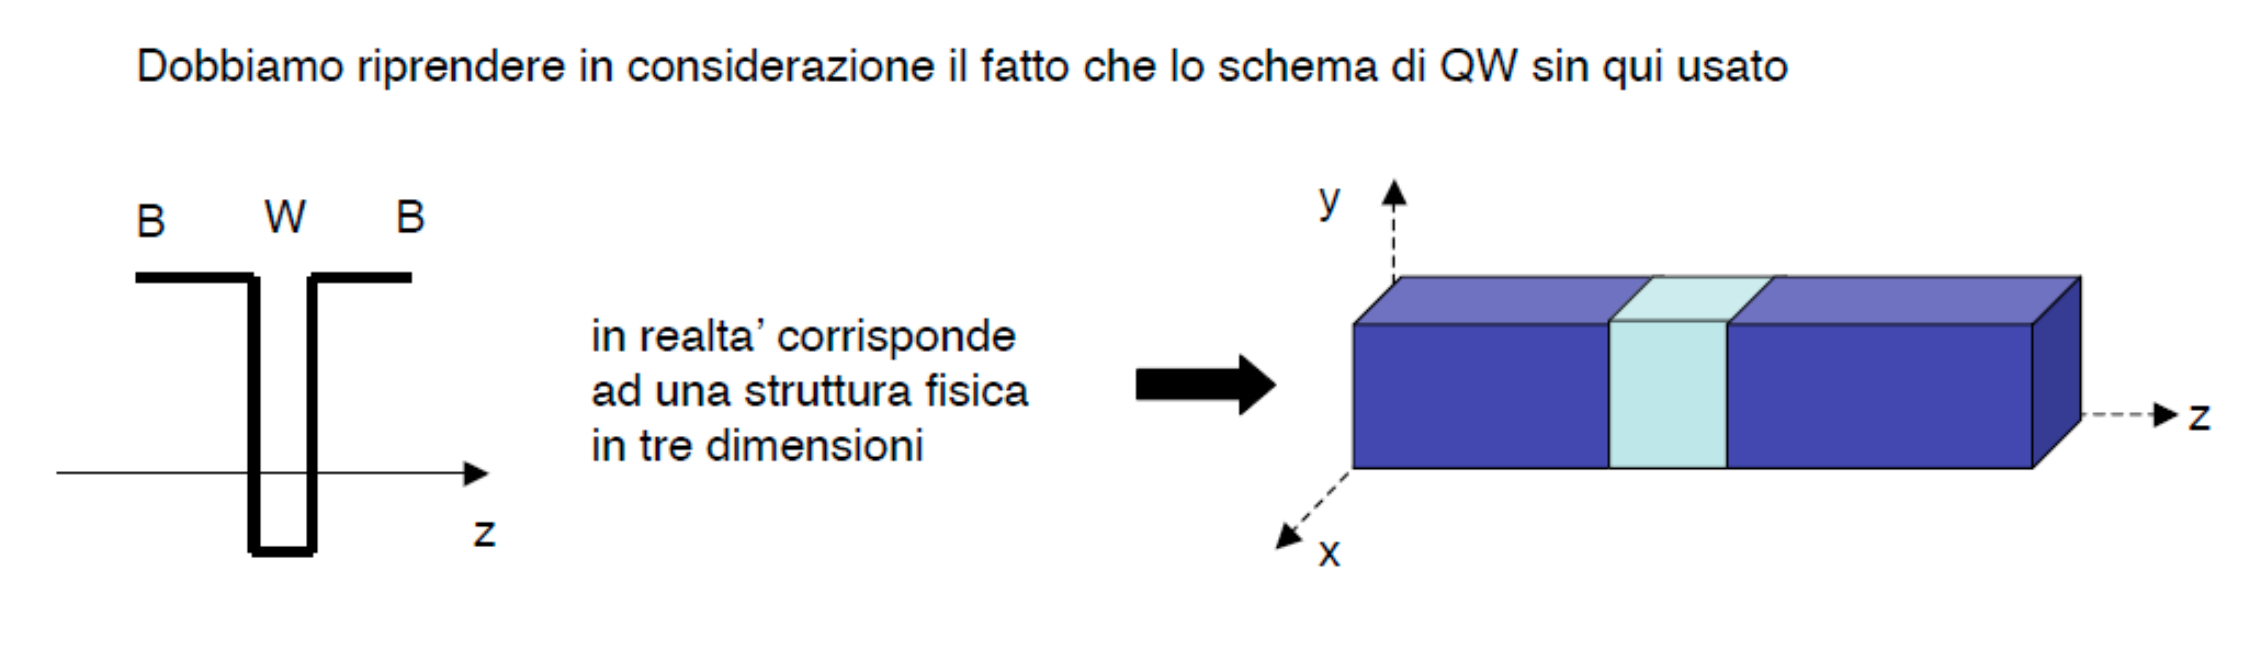
\includegraphics[width=1.1\linewidth]{images/9-Nanostrutture/IMG_1791.jpg}
\end{figure}

\textbf{Il problema completo corrisponde a considerare un'equazione agli autovalori in tre dimensioni in cui la variazione del potenziale avviene solo lungo una direzione $V(x,y,z) =V(z)$}, siccome l'elettrone è libero nel piano $(x,y)$, la soluzione generale avrà la forma: 
\[\psi(x,y,z) = e^{ik_x\cdot x} \cdot e^{ik_y\cdot y}\cdot u(z)\]
dove $u(z)$ soddisfa l'equazione unidimensionale:
\[
\left[-\frac{\hbar^2}{2m_e}\frac{d^2}{dz^2}+V(z)\right] u(z)= \varepsilon\, u(z),
\]
con
\[
\varepsilon = E - \frac{\hbar^2k_x^2}{2m_e} - \frac{\hbar^2k_y^2}{2m_e}.
\]
Gli autostati di $u(z)$ sono quelli determinati precedentemente, etichettati da un indice quantico $n$. L'energia totale dell'elettrone assume quindi la forma:
\[
E_n(k_x,k_y)= \varepsilon_n + \frac{\hbar^2}{2m_e}(k_x^2+k_y^2),
\]
e la funzione d'onda completa si scrive:
\[
\psi_{k_x,k_y,n}(x,y,z)= e^{ik_xx}\, e^{ik_yy}\, u_n(z).
\]
\begin{figure}[h]
\centering
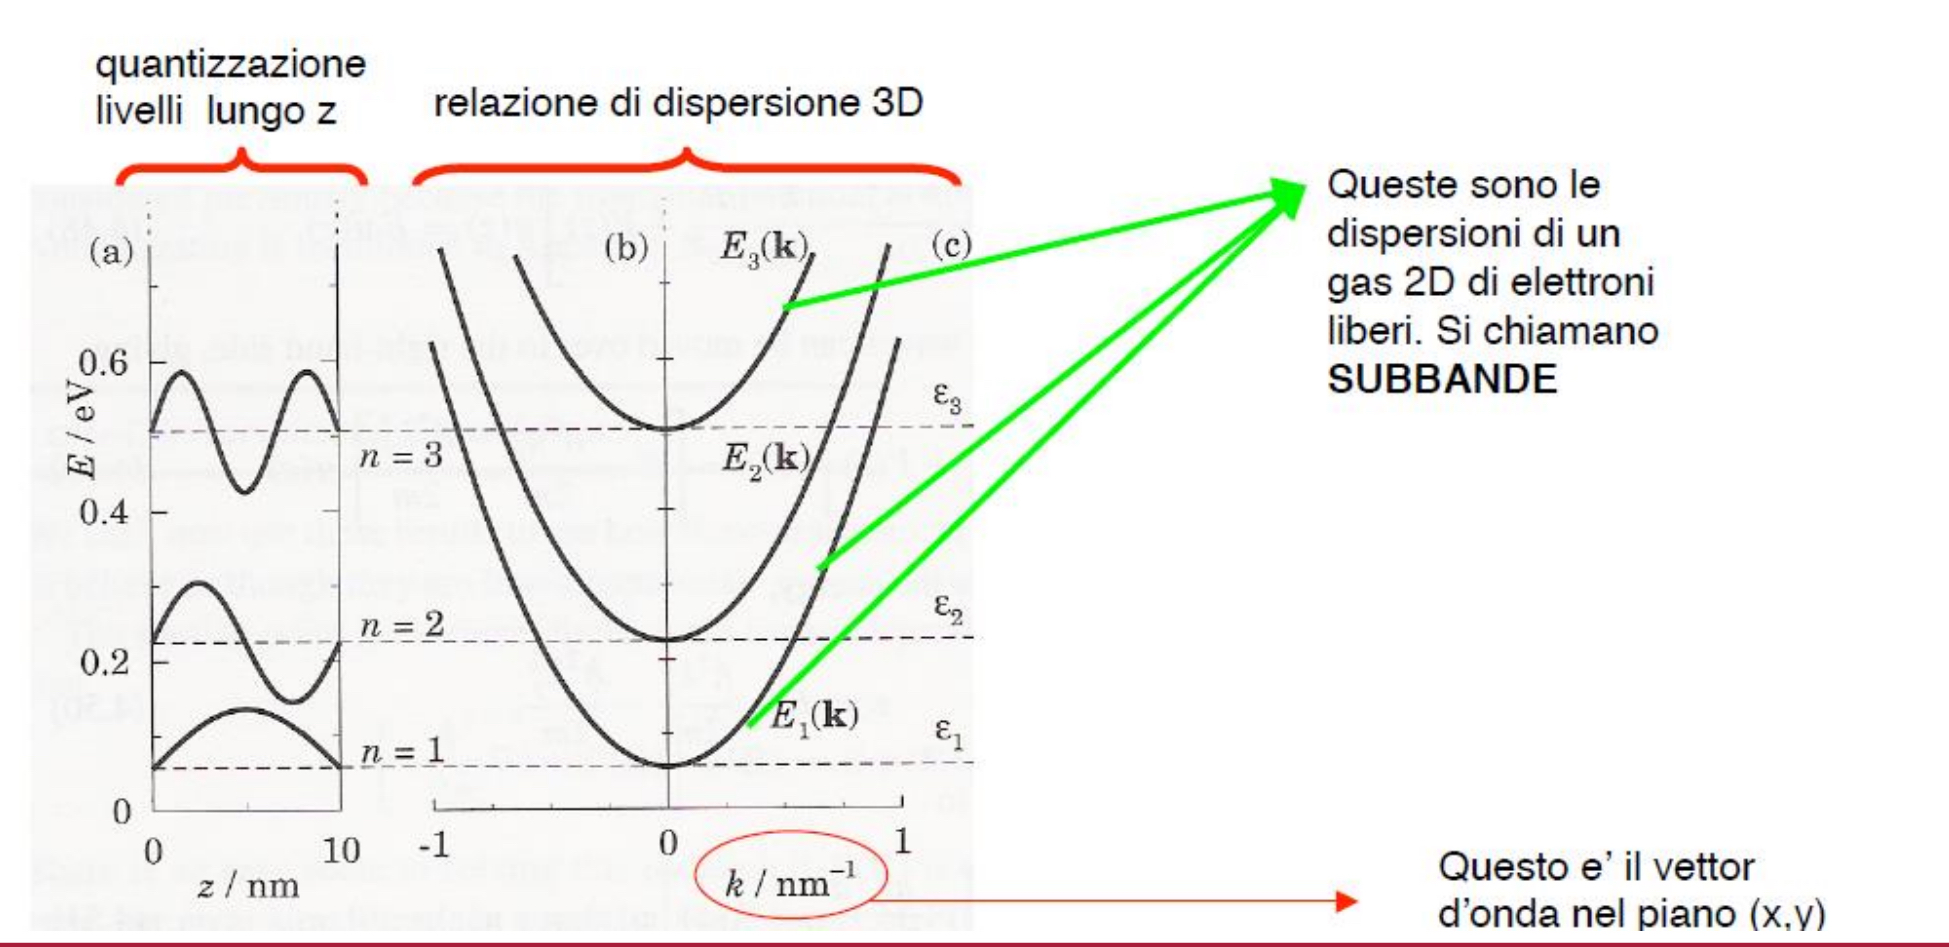
\includegraphics[width=\linewidth]{images/9-Nanostrutture/IMG_1792.jpg}
\caption{Profili delle funzioni d'onda estese.}
\end{figure}

\begin{figure}[h]
\centering
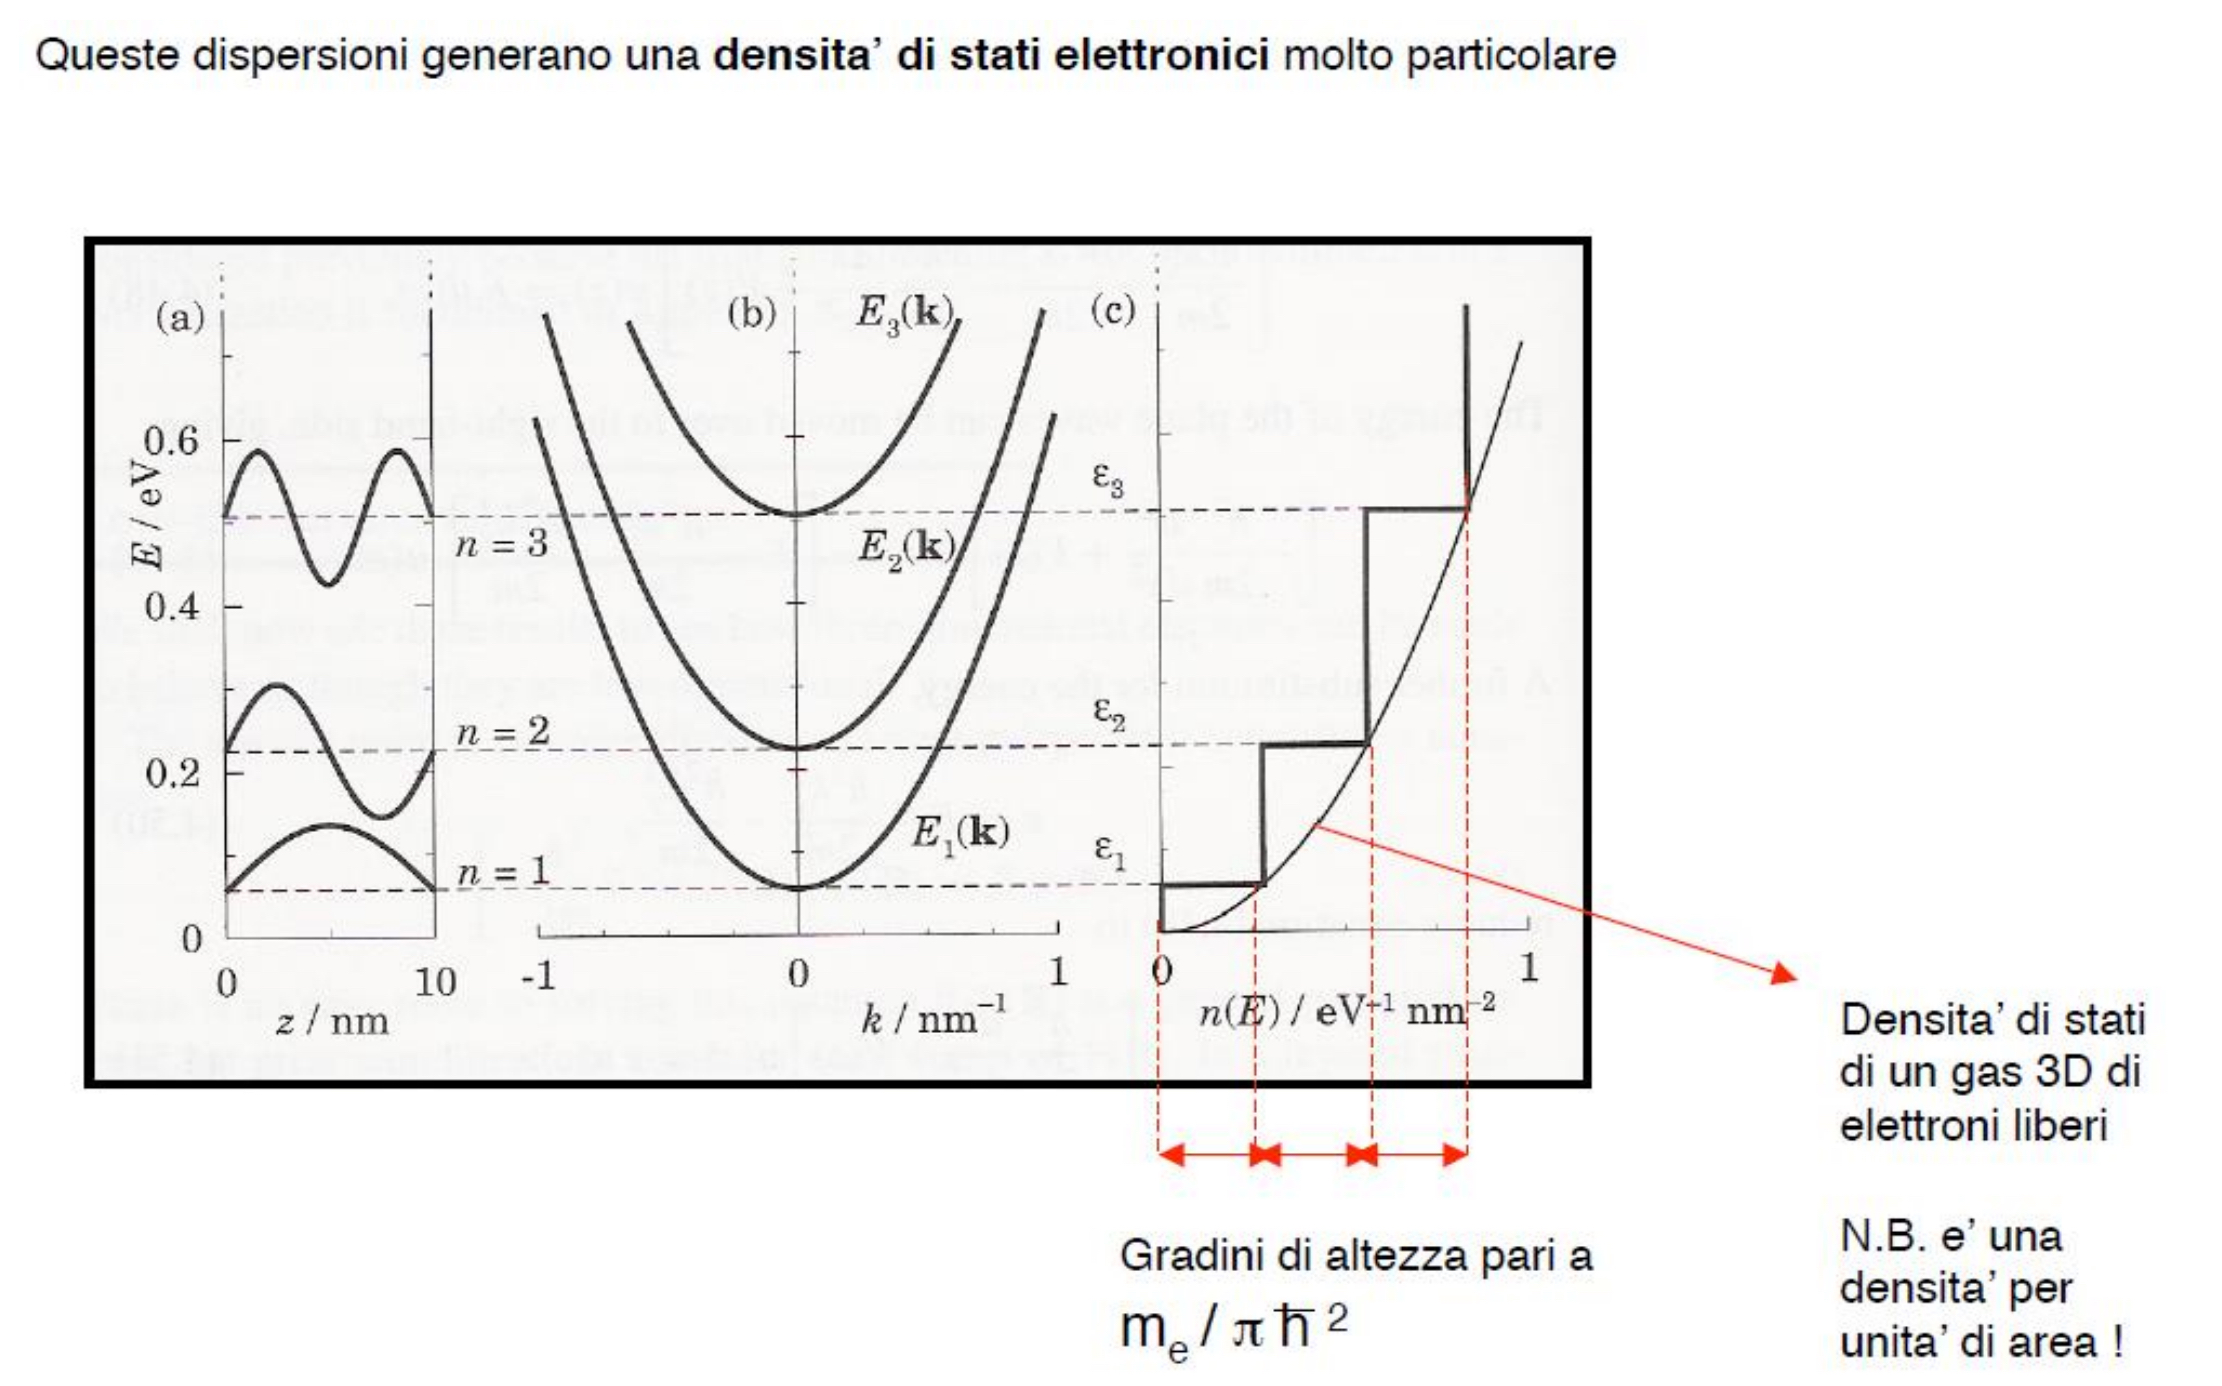
\includegraphics[width=\linewidth]{images/9-Nanostrutture/IMG_1793.jpg}
\caption{Ulteriore rappresentazione grafica del problema.}
\end{figure}